\documentclass[authoryear, 12pt,5p, times]{elsarticle}
%\usepackage[hypcap]{caption}
%\geometry{margin=0.95in,top=1.4in,bottom=1.4in}
\geometry{margin=1in,top=1.3in,bottom=1.3in}
\usepackage{float}
\usepackage{amsmath}
\usepackage[hidelinks]{hyperref} 
 \usepackage{gensymb}
\usepackage{subcaption}
\usepackage{url}
%\renewcommand\thefootnote{\fnsymbol{\dagger}}
\usepackage[symbol*]{footmisc}
\newcommand{\rpm}{\raisebox{.2ex}{$\scriptstyle\pm$}}
\begin{document}
%\footnote{This is a footnote}
\begin{frontmatter}
\title{Asteroid Astrometry from CCD Images}
\author{\today \\ \quad \\Jung Lin (Doris) Lee\\ dorislee@berkeley.edu\\Group partners: Jennifer Ito, Manuel Silvia\\Prof. James Graham, UGSI Heechan Yuk, Isaac Domagalski}
	\begin{abstract}
In this experiment,  we------
	\end{abstract}
\end{frontmatter}
\section{Introduction}
 
\section{Wavelength Calibration}
 We dark subtract the image 
 \begin{figure}[h!]
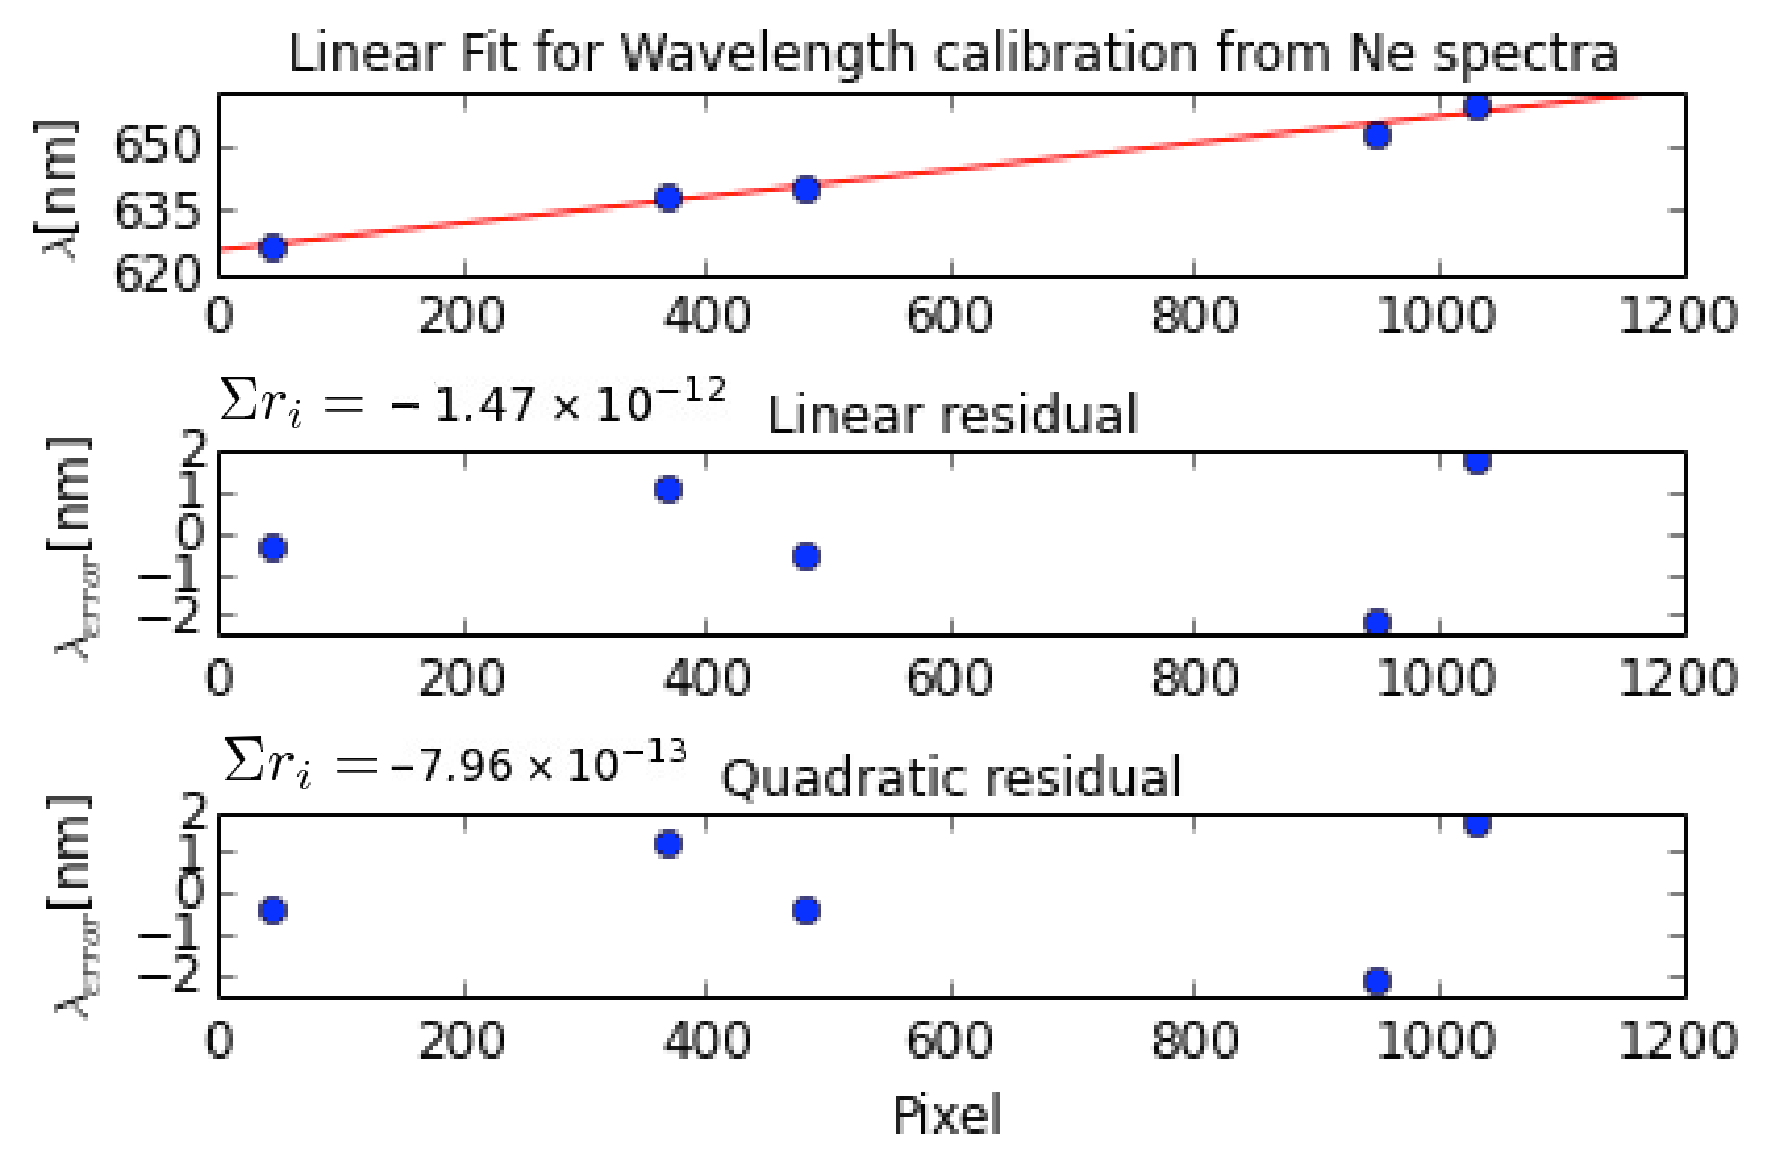
\includegraphics[width=0.5\textwidth]{figures/wavelength_calib}
\caption{The first order fit in the top figure shows that the dispersion is approximately linear ($\frac{d\lambda}{d\text{pixel}}$=0.0315 nm/pixel ). Since there is no notable pattern in linear residual, and the magnitude of the residual is small. From the bottommost quadratic figure, we see that the residual decrease by an order of magnitude.}
\label{calib}
\end{figure}
\section{Doppler Shift Determination}
\section{Conclusion}
 
 \section*{References}
 \begin{footnotesize}
 \begin{itemize}
\item Howell, Steve,  \textit{Handbook of CCD Astronomy}, 2nd Edition. Cambridge University Press, 2006.
%\item Wall, J. V. and Jenkins, C.R., \textit{Practical Statistics for Astronomers}, Cambridge University Press, 2002.
%\item Press, William H., and William T. Vetterling. \textit{Numerical Recipes in C: The Art of Scientific Computing}. Cambridge University Press, 1992. 
\item Chromey, Frederick R. \textit{To Measure the Sky: An Introduction to Observational Astronomy}. Cambridge: Cambridge UP, 2010. Print.
\item Stewart, James. \textit{Calculus: Early Transcendentals}. 7th ed. Belmont: Thomson/Brooks/Cole, 2003. Print.
\item Perryman, M.A.C. and Lindegren, L. and Kovalevsky, J. and Hoeg, E. and Bastian, U. and Bernacca, P.~L. and Cr{\'ez\'e}, M. and Donati, F. and Grenon, M. and Grewing, M. and van Leeuwen, F. and van der Marel, H. and Mignard, F. and Murray, C.A. and Le Poole, R.S. and Schrijver, H. and Turon, C. and Arenou, F. and Froeschl{\'e}, M. and Petersen, C.S.. The HIPPARCOS Catalogue. . p. L49-L52 1997
\item  Lindegren, L. and Babusiaux, C. and Bailer-Jones, C. and Bastian, U. and Brown, A.G.A. and Cropper, M. and Hog, E. and Jordi, C. and Katz, D. and van Leeuwen, F. and Luri, X. and Mignard, F. and de Bruijne, J.H. J. and Prusti, T.. The Gaia mission: science, organization and present status. . p. 217-223 2008
\end{itemize}
% \bibliography{references}
%\bibliographystyle{elsarticle-harv}
  \end{footnotesize}

\end{document}
